\subsection{Переменные звёзды}
\term{Переменные звёзды}~--- звёзды, у которых наблюдаются колебания блеска.   Для отнесения звезды к разряду переменных достаточно, чтобы блеск звезды хотя бы однажды претерпел изменение.

Переменные звёзды делятся на две большие группы: \imp{затменные} и \imp{физические}, причём физические подразделяются на \imp{пульсирующие} и \imp{эруптивные}.

К \term{пульсирующим} переменным  относят те звёзды, переменность которых вызвана процессами, происходящими в их недрах. Эти процессы приводят к периодическому изменению блеска звезды, а вместе с ним и других характеристик звезды~--- температуры поверхности, радиуса фотосферы и пр. Период переменности заключён в пределе от нескольких долей суток до нескольких лет. Абсолютную звёздную величину  и период связывает следующая формула:
\begin{equation}
	M = -1.01^m - 2.97\lg T,
\end{equation}
где $T$~--- период, выраженный в сутках, а $M$~--- абсолютная звёздная величина.

Классический пример пульсирующих переменных звёзд --- цефеиды.

\begin{figure}[h!]
\begin{center}
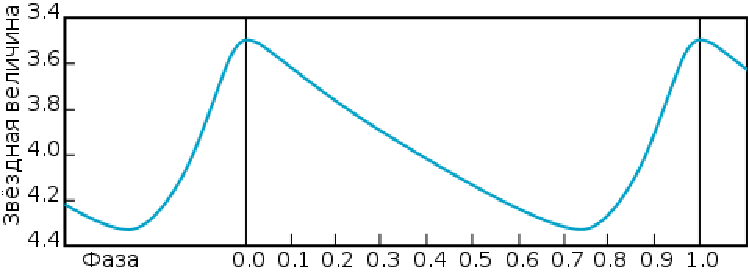
\includegraphics[width=0.7\tw]{var-stars}
\caption{Кривая блеска $\delta$ Цефея}
\end{center}
\end{figure}

К \term{эруптивным} переменным звёздам относятся звёзды, меняющие свой блеск нерегулярно или единожды за время наблюдений. Все изменения блеска эруптивных звёзд связывают с бурными процессами и вспышками в их хромосферах и коронах.

\term{Затменно-переменные} звёзды --- системы из двух звёзд, суммарный блеск которых периодически изменяется с течением времени. Причиной изменения блеска могут быть затмения звёзд друг другом, или изменение их формы взаимной гравитацией в тесных системах.

На всех кривых блеска (Рис.~\ref{var-stars}) заметны два минимума: глубокий (главный), соответствующий затмению главной звезды спутником, и слабый (вторичный), возникающий, когда главная звезда затмевает спутник.

%\begin{figure}[h!]
%	\centering
%	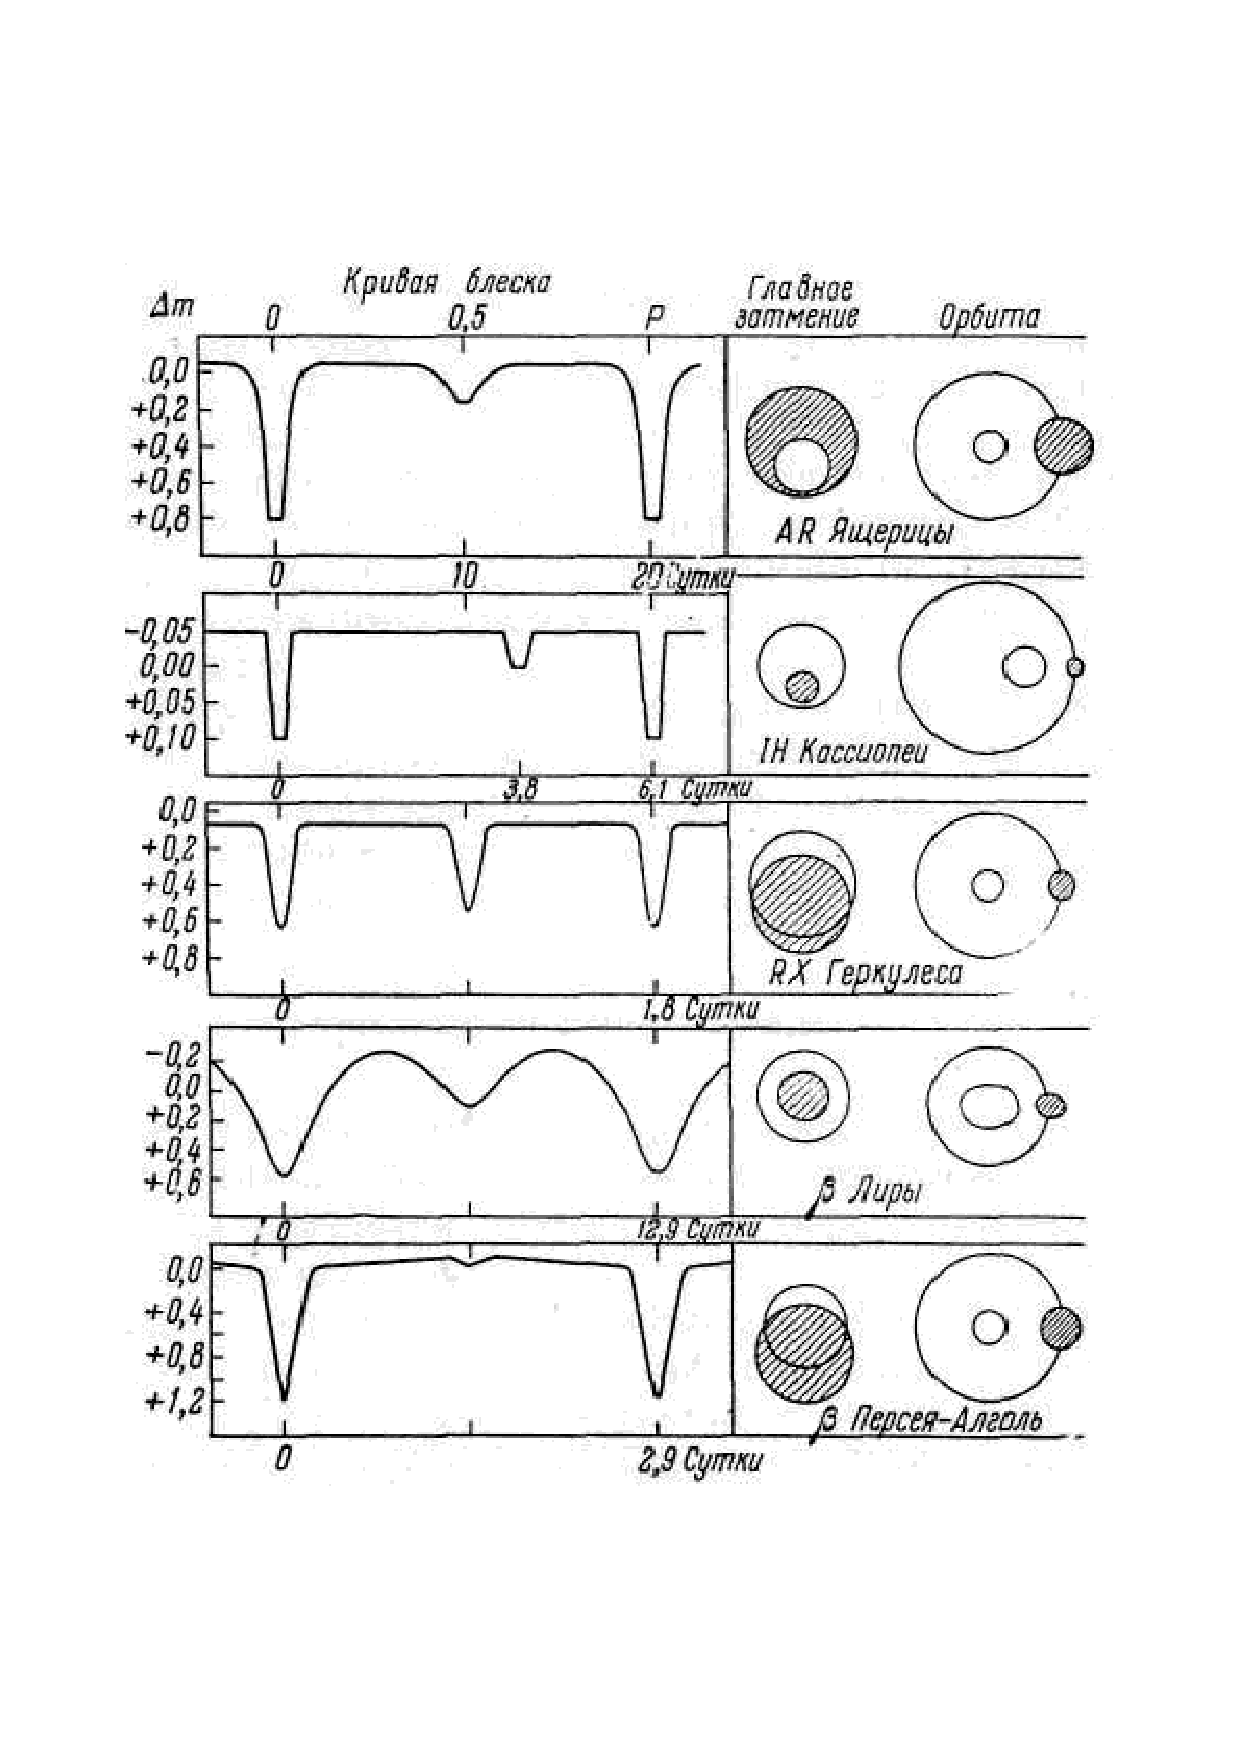
\includegraphics[width=0.8\tw]{var-stars2}
%	\caption{Кривые блеска некоторых затменно-переменных звёзд}
%	\label{var-stars}
%\end{figure}

\begin{figure}[!h]
\centering
 \begin{tikzpicture}
 \begin{axis}[
 no markers,
% xlabel={Прямое восхождение $\alpha^h$}, 
% ylabel={Склонение $\delta^{\circ}$},
 minor x tick num = 1,
 minor y tick num = 1,
 grid = both,
 line width=.7pt, 
% extra y ticks={23.44, -23.44},
 ymax=1.02,
 ymin=0.65,
 xmax=1,
 xmin=0,
% xtick={0,4,8,12,16,20,24}
 ]
% \addplot [domain=0:24, samples=100]{atan(sin(x*15)*tan(23.44))}; 
	\addplot table{data/light-curve-W-UMa.txt};
 \end{axis}
 \end{tikzpicture}
 \caption{График зависимости склонения от прямого восхождения Солнца}
\end{figure}



